\documentclass[11pt,twoside,openright]{article}
\usepackage[pdftex]{color,graphicx,thumbpdf}
\usepackage[pdftex,pdfstartview=FitH,breaklinks,linktocpage]{hyperref}
\usepackage[T1]{fontenc}
\usepackage[utf8]{inputenc}
\usepackage[french]{babel}
\usepackage{amsmath}
\usepackage{amsfonts}
\usepackage{graphicx}
\usepackage{subfigure}
\usepackage{tikz}
\usepackage{booktabs}
\usepackage{multirow}
\usepackage{xcolor}

\def\code#1{\texttt{#1}}

\usepackage[top=2cm, bottom=2cm, left=2cm, right=2cm]{geometry}

\pdfminorversion=4

\makeatletter
\addto\captionsfrench{\def\tablename{{\scshape Tableau}}}
\makeatother

\setlength{\parskip}{0.5em}

\begin{document}


\renewcommand{\thepage}{}
% \include{PagesCouv/pg}`

\renewcommand{\thepage}{\arabic{page}}
\setcounter{page}{1}

% ==================================================================
% DIFFÉRENTS LISTES
% table des matières générale
\tableofcontents
\newpage
\section{Contexte et objectifs}
Maladie infectieuse émergente, apparue en Chine continentale, à la fin de l'année 2019, la COVID-19 (maladie à coronavirus 2019) a provoqué une crise sanitaire et économique majeure. En l'état actuel de nos connaissance, le diagnostic précoce de cette maladie demeure un des meilleurs moyens de lutter contre sa propagation. 

Dans le cadre du développement de moyens de détection rapides et sûrs de la maladie, l'objectif de ce projet est de créer une intelligence artificielle capable de détecter la présence de la COVID-19 chez un patient, à partir d'une radiographie pulmonaire. Cette technique pourrait être l'un des moyens les plus rapide et efficace pour diagnostiquer cette maladie, en milieu hospitalier.

Pour développer cette intelligence artificielle, nous nous baserons principalement sur des techniques de réseaux de neurones, et plus spécifiquement, les réseaux de neurones convolutifs (CNN). Ces techniques ont montré leurs efficacités pour la classification des images.

L'entraînement de ces algorithmes de machine learning se base sur un jeu de données constitué de milliers de radiographies pulmonaires. 
Ces clichés radiographiques de patients sont de trois types: 
\begin{itemize}
 	\item des radiographies de patients détectés positifs à la COVID-19 
    \item des radiographies de patients sains
    \item des radiographies de patients atteint de pneumonies virales, autres que la COVID-19
\end{itemize}

L'objectif de ce travail est donc d'entraîner, à partir du jeu de données dont nous disposons, une intelligence artificielle capable de distinguer les trois cas (COVID-19, normal et viral). Pour atteindre cet objectif, nous distinguons principalement deux grandes étapes :
\begin{itemize}
    \item l'exploration, l'analyse et la visualisation de données constituent la première étape du projet. Cette étape permettra d'examiner le format et la qualité des données, d'identifier des biais dans ces données, etc...
    \item la deuxième étape consiste à mettre en place des algorithmes de classifications qui se basent sur les réseaux de neurones. Plusieurs algorithmes, plus ou moins complexes, seront par la suite testés et évalués. 
\end{itemize}
\newpage
\section{Données}

Les données exploitées dans ce travail sont des images de ragiographies pulmonaires, disponibles sur le site kaggle (https://www.kaggle.com/tawsifurrahman/covid19-radiography-database). Ces images sont regroupées en trois classes : COVID-19, normal et viral-pneumonia, pour des personnes qui sont respectivement, atteintes de la COVID-19, saines et atteintes de pneumonie virale.  

\subsection{Nombre d'images par classe}

Nous disposons d'un jeu de données équilibré entre les trois classes. La figure~\ref{fig:nb_classes}, qui montre le nombre d'images pour chacune des trois classes, permet d'illustrer cet équilibre. 

\begin{figure}[htbp]
\centering
\includegraphics[width=12cm]{nombre_classes.png}
\caption{Nombre d'images par classe}
\label{fig:nb_classes}
\end{figure}

\subsection{Taille et encodage des images}
En termes de format de données, les images exploitées dans ce projet sont différentes par deux aspects :
\begin{itemize}
    \item Nombre de pixels : le nombre de pixels suivant les deux directions varie d'une image à l'autre;
    \item Encodage : bien que les images exploitées soient, visuellement, en niveau de gris, certaines sont encodées en niveau de gris et d'autres en RGB. 
\end{itemize}

La figure~\ref{fig:im_size_enc} montre des tableaux qui regroupent, pour chacune des trois classes, le nombre d'images par type d'encodage et par nombre de pixels suivant les deux dimensions.

\begin{figure}[htbp]
  \centering
  \subfigure[COVID-19] {
    \includegraphics[width=9cm]{covid_size.PNG}
    \label{fig:covid}
  }
  \subfigure[Normal] {
    \includegraphics[width= 9cm]{normal_size.PNG}
    \label{fig:normal}
  }
  \subfigure[Pneumonie virale] {
    \includegraphics[width= 9cm]{VP_size.PNG}
    \label{fig:Pneumonie-virale}
  }
  \caption{Pour chaque classe : nombre d'images par type d'encodage et par nombre de pixels suivant les deux dimensions.}
  \label{fig:im_size_enc}
\end{figure}

\section{Analyse et statistiques sur les images}
L'objectif de cette partie est d'analyser les radiographies, afin d'identifier les différences entre les images, et de détecter des biais le cas échéant.

\begin{figure}[htbp]
\centering
\includegraphics[width=8cm]{COVID-19 (366).png}
\caption{Exemple d'une ragiographie COVID-19}
\label{fig:Radio_COV}
\end{figure}

\subsection{Première analyse visuelle}

Une première analyse visuelle est effectuée en parcourant des images pour les trois classes. Nous observons, sur quelques radiographie, la présence de certains appareils médicaux de mesures, de forme filaire ou tubulaire. \textbf{Ces dispositifs médicaux sont d'avantage présents dans les radiographies de type COVID-19, ce qui peut créer un biais lors de la classification}.  


\subsection{Statistiques sur les images}

Afin d'analyser la répartition des niveaux de gris, nous allons analyser la distribution de la moyenne et de l'écart-type de ces niveaux de gris dans les images de chacune des classes. La figure~\ref{fig:Histos_gray_level} montre la distribution des moyennes et écart-types pour les trois classes. Nous constatons que:
\begin{itemize}
\item La dispersion des moyennes et des écart-types des niveaux de gris est importante. Cette dispersion est plus accentuée pour les images de types COVID-19 et Viral Pneumonia.
\item Contrairement aux autres images, les images de type COVID-19 ont tendance à avoir une moyenne plus élevée et un écart-type plus faible. Dans ce qui suit, nous allons tenter d'identifier la cause de cette différence.
 \end{itemize}

\begin{figure}[htbp]
\centering
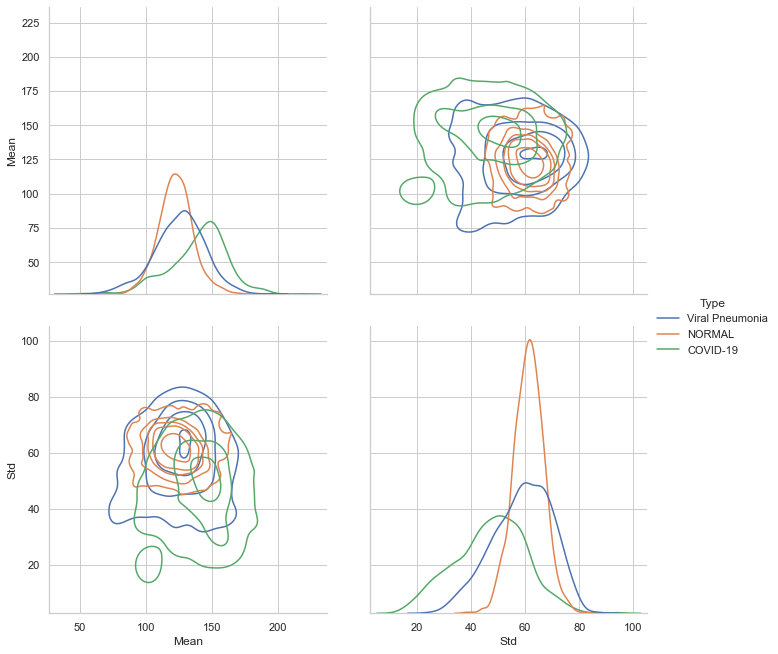
\includegraphics[width=14cm]{Histos_gray_level.png}
\caption{Distribution des moyennes et écart-types pour les trois classes.}
\label{fig:Histos_gray_level}
\end{figure}

\subsection{Filtrage des pixels les moins pertinents}
Nous proposons de filtrer les pixels les moins pertinents pour la classification des images. Nous utilisons pour cela la classe \code{SelectPercentile} de \code{Sklearn.feature\_selection}. La figure~\ref{fig:filtrage} montre un filtrage des pixels en utilisant différents pourcentages de pixels filtrés. Dans les six images présentées dans la figure, les pixels blancs correspondent aux pixels filtrés.
\begin{figure}[htbp]
\centering
\includegraphics[width=18cm]{Filtrage.png}
\caption{Filtrage des pixels les moins pertinents}
\label{fig:filtrage}
\end{figure}

Légitimement, nous pensions que les bords des radiographies étaient peu porteurs d'informations.
Cependant, dans la figure~\ref{fig:filtrage}, les bords verticaux de l'image ne sont toujours pas éliminés, même avec un paramétrage fixé à 70 \%.
Nous verrons que dans le paragraphe suivant que cela est dû à un biais sur les images.

\subsection{Biais sur les images de type COVID-19}
Une analyse poussée des images a permis d'identifier un deuxième biais (autre que le biais des équipements médicaux) : les images de type COVID-19 contiennent moins de bords noirs. Ces radiographies ont fait l'objet d'un pré-traitement, le "zoom". 
Nous avons pu remarquer ce biais en appliquant deux modèles de visualisation d'images : le modèle Isomap et le modèle TSNE. Les résultats de la visualisation de ces deux modèles sont présentés dans le fichier \code{datavisualisation.ipynb}.

\begin{figure}[htbp]
  \centering
  \subfigure[COVID-19] {
    \includegraphics[width=5cm]{COVID-19 (1).png}
    \label{fig:covid1}
  }
  \subfigure[COVID-19] {
    \includegraphics[width=5cm]{COVID-19 (20).png}
    \label{fig:covid2}
  }
  \subfigure[COVID-19] {
    \includegraphics[width=5cm]{COVID-19 (60).png}
    \label{fig:covid3}
  }
  \subfigure[Normal] {
    \includegraphics[width= 5cm]{NORMAL (1).png}
    \label{fig:normal1}
  }
  \subfigure[Normal] {
    \includegraphics[width= 5cm]{NORMAL (20).png}
    \label{fig:normal2}
  }
  \subfigure[Normal] {
    \includegraphics[width= 5cm]{NORMAL (60).png}
    \label{fig:normal3}
  }
  \subfigure[Pneumonie virale] {
    \includegraphics[width= 5cm]{Viral Pneumonia (1).png}
    \label{fig:PV1}
  }
    \subfigure[Pneumonie virale] {
    \includegraphics[width= 5cm]{Viral Pneumonia (20).png}
    \label{fig:PV2}
  }
  \subfigure[Pneumonie virale] {
    \includegraphics[width= 5cm]{Viral Pneumonia (60).png}
    \label{fig:PV3}
  }
  \caption{Comparaison d'images prises au hasard parmi les trois classes.}
  \label{fig:comp_vis}
\end{figure}


Ce biais est cohérent avec ce que nous avons observé pour le filtrage des pixels les moins pertinents (figure~\ref{fig:filtrage}) et dans les distributions (figure~\ref{fig:Histos_gray_level}) :
\begin{itemize}
    \item Les bords verticaux des images ne sont pas éliminés lors du filtrage (figure~\ref{fig:filtrage}), car ils participent fortement à distinguer les images de type COVID-19 des autres images.
    \item Dans les distributions (figure~\ref{fig:Histos_gray_level}), les images de COVID-19 ont des moyennes plus élevées et des écart-types plus faibles, ce qui est un effet de l'absence des bords noirs. Cette absence induit une augumentation du niveau de gris moyen, et une diminution de l'hétérogénéité de l'image et donc de son écart-type de niveau de gris.
\end{itemize}


\subsection{Bilan}

La visualisation et l'analyse des données nous a permis de constater que les images de type COVID-19 diffèrent des autres images par deux aspects : 
\begin{itemize}
    \item La présence plus fréquente de certains appareils médicaux de mesures, de forme filaire ou tubulaire;
    \item et l'absence de bords noirs verticaux, résultant probablement d'un zoom effectué par les émetteurs de ces images.
\end{itemize}

Ces caractéristiques risque d'induire en erreur un modèle prédictif, qui se baserait en partie sur une reconnaissance liée à celles-ci.

Il est possible de corriger la deuxième différence, en effectuant une opération de pré-traitement des images avant de les utiliser pour l'entraînement des modèles. Cette opération consiste à éliminer les bords noirs verticaux sur toutes les radiographies. Ainsi, le modèle se concentrera mieux sur les différences de caractéristiques aux niveaux des poumons.

\section{Modélisation}

Dans cette partie, nous proposons différents modèles pour la classification des images. Ces modèles se basent sur les réseaux de neurones convolutifs.

Les différentes modélisations abordées dans ce projet sont les suivantes :
\begin{itemize}
\item Modélisation 1: CNN Lenet.
\item Modélisation 2: CNN personnalisé
\item Modélisation 3: Transfer Learning avec EfficientNetB5
\item Modélisation 4: Feature extraction avec InceptionV3 et Xgboost.
\item Modélisation 5: VGG16 avec augmentation d'image.
\end{itemize}

Avant de détailler les modèles, il convient de décrire le pré-traitement effectué sur les images et la métrique qui sera utilisée pour l'évaluation des modèles.

\subsection{Pré-traitement des images}

\paragraph{Traitement des bords verticaux noires} 

Lors de la phase de datavisualisation, l'équipe projet à constaté que les radiographies de type COVID ne présentaient pas de bords noirs latéraux, tandis que les radiographies de type Normal et Pneumonie en présentaient.  
L'application d'un traitement d'image peut atténuer le biais induit par la présence de bords noirs verticaux.
L'idée sous-jacente, est de réaliser un «zoom» sur les radiographie NORMAL et PNEUMONIE.
La solution retenue, préconise l'élimination des bords latéraux, inférieurs et supérieurs, afin de se focaliser sur l'information utile, les poumons. La partie basse des radiographies, correspondant aux coupoles diaphragmatiques est éliminée car peu porteuse d'informations. Il en est de même pour la partie haute des radiographies, correspondant à la région du corps située au dessus des clavicules. Les parties latérales sont éliminés car elles constituent l'arrière plan de la radiographie.

\paragraph{Redimensionnement et normalisation des images} 
Un traitement est ensuite nécessaire pour avoir des images de même dimension. Ceci est nécessaire pour l'entraînement des modèles. La taille choisie pour tous les images est de 256X256 pixels.

Pour un meilleur entrainement des modèles, une bonne pratique consiste à normaliser toutes les images,  en divisant le niveau de gris de chaque pixel par 255, cette valeur étant le niveau de gris maximal.

\subsection{Métriques et sorties des modèles}

\paragraph{Fonction de pertes}
La fonction de perte est la valeur que l'algorithme cherchera à minimiser. Dans notre cas, nous utilisons la fonction \code{categorical\_crossentropy} adapté pour une problématique de classification multi-classes. 

\paragraph{Métrique}
La métrique qui nous intéresse est la précision \code{accuracy}. Elle correspond au pourcentage des bonnes prédictions.

\paragraph{Sortie des modèles}
La sortie des modèles correspond à la probabilité d'une image d'appartenir à chacune des trois classes. Par la suite, nous attribuons à l'image, la classe qui a la probabilité la plus élevée.



\subsection{Modèle LeNet}

Cette première modélisation fait appel à une architecture basée sur "LeNet", un réseau de neurones convolutif, caractérisé par une alternance de couche de convolution et de pooling, permettant l'extraction des caractéristiques des radiographies. La classification est assurée par une couche dense de réseau de neurones connectés.

\subsection{Modèle personnalisée}

Cette deuxième modélisation est un modèle personnalisé par l'équipe, caractérisé par une alternance de couche de convolution et de pooling, permettant l'extraction des caractéristiques des radiographies. La classification est assurée par une couche dense de réseau de neurones connectés.

\subsection{EfficientNetB5}

Cette troisième modélisation est basé sur le principe du transfer learning, qui consiste à utiliser un modèle pré-entrainé sur des centaines de milliers d'image. Le modèle pré-entrainé choisi est EfficientNetB5, il permet l'extraction des caractéristiques des radiographies. La classification est assurée par une couche dense de réseau de neurones connectés.
Afin d'améliorer la performance de notre modèle, une opération de fine tuning a permis d'adapter les 3 dernières couches de convolutions du modèles pré-entrainé, à nos données. Ce réglage fin permet un  nouveau calcul des poids synaptiques et donc une meilleure extraction des caractéristiques des radiographies.

\subsection{InceptionV3}

Cette quatrième modélisation combine les techniques de deep learning et de machine learning "classique". Un modèle pré-entrainé, InceptionV3, est utilisé pour extraire les caractéristiques des radiographies et un XGBoostClassifier est utilisé pour opérer la classification en sortie du modèle pré-entrainé.

\subsection{VGG16 avec augmentation d'image}

Cette dernière modélisation utilise la technique d'augmentation d'image qui permet d'enrichir le jeu de données et de réduire le phénomène d'overfitting. VGG16, un modèle pré-entrainé, est utlisé pour extraire les caractéristiques des radiographies. La classification est assurée par une couche dense de réseau de neurones connectés.
Combiner à une opération de fine tuning sur les 4 dernières couches du modèle VGG16, le modèl s'avère performant dans ses constitue prédctions.

\subsection{Résultats des différents modèles}

\subsection{Bilan}

\section{Conclusion}

\end{document}
